\chapter{Fourier Transform} 
\section{Introduction}
\label{sec:Introduction}
The Fourier transform is a representation of a temporal signal. Why would we want to
represent a signal in another space and why use FT? The FT has wonderful properties that
allow us to easily handle convolution or derivation in the frequency space. The $
\mathscr{ FT } $ can handle non periodic signals.

\subsection{Non-rigorous development of the $ \mathscr{ FT }  $}
\label{subsec:Non-rigorous development of the $ \mathscr{ FT }  $}
We begin by recalling the definiton of a Fourier series for a function $ f $ defined on
the interval $ =l \leq x \leq l $ and we let $ l $ go to infinity. 
\begin{equation}
f(x) = \sum_{n=\infty}^{\infty} C_n e^{ in\pi x / l} 
\label{eq:fs_rep}
\end{equation}

which gives us 
\[
    C_n = \frac{ 1 }{ 2l } \int\limits_{-l}^{l} f(t) e^{ -in\pi t / l} \ dt 
\]
If $ f $ is defined on the entire real line then we can take l to infinity and see how it
affects the formulas.
Substituting the expression of $ C_n $ into \ref{eq:fs_rep} we obtain 
\begin{align*}
    f(x)  &= \lim_{l \to \infty} \left[ \sum_{n=\infty}^{\infty} \left( \frac{ 1 }{ 2l }
    \int\limits_{-l}^{l} f(t) e^{ -in\pi t / l } \ dt\right) e^{ in\pi x / l}  \right]  \\ 
          &= \lim_{l\to \infty} \left[ \sum_{n=-\infty}^{\infty} \frac{ 1 }{ 2l }
          \int\limits_{-l}^{l} f(t) e^{ in\pi(x-t) / l} \ dt   \right]  \\ 
\end{align*}
We want to transform this into a Riemann sum formulation of an integral.
Thus, we partition l using our infinite sum by letting 
\[
    \lambda_n = \frac{ n\pi }{ l } \quad \text{ and } \quad \Delta \lambda = \lambda_{n+1}
    - \lambda_n = \frac{ \pi  }{ l } 
\]
This gives us, $ \frac{ 1 }{ 2l  } \cdot \frac{ \pi }{ \pi } = \frac{ 1 }{ 2\pi } \cdot
\Delta\lambda   $ and 
\begin{equation} 
    f(x) = \lim_{l\to \infty}  \sum_{n=-\infty}^{\infty} \left[\frac{ 1 }{ 2\pi }
          \int\limits_{-l}^{l} f(t) e^{ \lambda_ni(x-t) } \ dt   \right]  \Delta \lambda
    \label{eq:towards_riemann}
\end{equation}
we denote the inner expression as 
\begin{equation}
    F_l(\lambda) = \frac{ 1 }{ 2\pi  } \int\limits_{-l}^{l} f(t) e^{ \lambda i (x-t) } \
    dt 
    \label{eq:Fllam}
\end{equation} 
and this with \ref{eq:towards_riemann} we have 
\[
    \sum_{-\infty}^{\infty} F_l(\lambda_n) \Delta\lambda 
\]
which is similar to the definition of a riemann sum for the integral 
\[
    \int\limits_{-\infty}^{\infty} F_l(\lambda) \ d\lambda 
\]
As $ l \to \infty, \ \Delta \lambda \to 0  $ so $ \Delta \lambda  $ becomes $ d\lambda  $
and \ref{eq:towards_riemann} becomes 
\[
    f(x) = \lim_{l\to\infty} \int\limits_{-\infty}^{\infty} F_l(\lambda) \ d\lambda 
\]
As $ l \to \infty, \ \ref{eq:Fllam} $ becomes 
\begin{equation}
    \frac{ 1 }{ 2\pi } \int\limits_{-\infty}^{\infty} f(t) e^{ i\lambda(x-t)} \ dt
    \label{eq:fllaminft} 
\end{equation} 
which gives us 

\[
    \frac{ 1 }{ 2\pi } \int\limits_{-\infty}^{\infty}   \int\limits_{-\infty}^{\infty} 
    f(t) e^{ i\lambda(x-t)} \ dt \ d\lambda 
\]

which is 
\begin{equation}
    f(x) = \frac{ 1 }{ \sqrt{2\pi}  } \int\limits_{-\infty}^{\infty} \left( \frac{ 1 }{
    \sqrt{2\pi}  } \int\limits_{-\infty}^{\infty} f(t) e^{ -i\lambda t} \ dt\right) e^{
i\lambda x} \ dx 
    \label{eq:expanded}
\end{equation}
We denote 
\[
    \widehat{f}(\lambda) = \frac{ 1 }{ \sqrt{2\pi}  } \int\limits_{-\infty}^{\infty} f(t)
    e^{ -i\lambda t } \ dt 
\] 
and we now have 
\[
    f(x) = \frac{ 1 }{ \sqrt{2\pi}  } \int\limits_{-\infty}^{\infty} \widehat{f}(\lambda)
    e^{ i\lambda x} \ d\lambda 
\]

This now allows us to define the Fourier transform. 
\section{Fourier Transform in $ \mathscr{ L } ^1\left( \mathbb{R}\right)  $}
\label{sec:Fourier Transform in $ \mathscr{ L } ^1\left( \mathbb{R}\right)  $}
Assume $ f \in \mathscr{L}^1 \left( \mathbb{R}\right)  $ where 
\[
    \mathscr{ F } f\left( \lambda \right) = \widehat{f}\left( \lambda \right) =  
    \int\limits_{-\infty}^{\infty} f(t) e _{  }^{ -2i\pi
\lambda t} \ dt
\]
We also have 
\[
    \overline{\mathscr{ F }} f\left( \lambda \right) = \int\limits_{-\infty}^{\infty} f(t) 
    e _{  }^{ 2i\pi\lambda t} \ dt
\]
$ \mathscr{ F } f\left( \lambda\right)  $ is defined for $ f\in \mathscr{ L } ^1\left(
\mathbb{R}\right)  $. We introduce the notation 
\[
h(\lambda, x) = f(t) e _{  }^{ -2i\pi\lambda t } 
\]
For $ \lambda $, we have $ \left | h(\lambda, t)  \right | \leq \left | f(t)  \right |  $
and $ \left | f \right |  $ is integrable. 
\[
\lambda \to h(\lambda, t) \text{ is continuous } 
\]
Applying the theorem of continuous? we have 
\[
\lambda \to \int\limits_{ }^{ } h(\lambda, t) \ dt \ \text{ is continuous } 
\]
We continue ? 
\[
\frac{ dh(\lambda, t)  }{ d\lambda  } = -2i\pi t h(\lambda, t) 
\]

\[
\left| \frac{ dh(\lambda, t)  }{ d\lambda  } \right| \leq  2\pi\left|  t h(\lambda, t)
\right| \leq 2\pi \left | t f(t)  \right |  
\]
If $ \left | tf(t)  \right |  $ is in $ \mathscr{ L } ^1( \mathbb{R})$ we can apply the
theorem of derivation and we have 
\[
\frac{ d \mathscr{ F } f(\lambda)  }{ d\lambda  } = \frac{ d }{ d\lambda  } \int\limits_{ }^{ }  h(\lambda, t) 
= \int\limits_{ }^{ } \frac{ d }{ d\lambda  } h(\lambda, t) = \int\limits_{ }^{}-2i\pi t
f(t) e _{  }^{ -2i\pi\lambda t  } \ dt = \widehat{-2i\pi t f(t)} \left( \lambda \right)  
\]

\begin{defn}[]
    \[
        \widehat{f}\left( \lambda \right) = \mathscr{ F } f(\lambda ) = \int\limits_{ }^{ }
        e _{  }^{ -2i\pi\lambda t } f(t) \ dt
    \]
    \label{def:}
\end{defn}

\begin{ftheo}[Riemann-Lebesgue]
    Let $ f \in \mathscr{ L } ^1( \mathbb{R})    $ and let 
    \[
        \mathscr{ F } f(\lambda) = \widehat{f}\left( \lambda \right) = \int\limits_{ }^{ }
        f(t) e _{  }^{ -2i\pi \lambda t } \ dt
    \]
    \begin{enumerate}
        \item $ \widehat{f}\left( \lambda\right)  $is continuous and bounded 
        \item The operator $ \mathscr{ F }  $ is continuous linear from $ L^1( \mathbb{R})
            $ to $ \mathscr{ L } ^{\infty} ( \mathbb{R})  $ and 
            \[ \| \widehat{f}  \|^{ }_{\infty} \leq \| f \|^{ }_{ 1}  \]
        \item \[
                \lim _{ \left | \lambda  \right | \to \infty  }^{  } \left | \widehat{f}
                \left( \lambda \right) \right | = 0
        \]
    \end{enumerate}
    \label{th:Riemann-Lebesgue}
\end{ftheo}

\begin{enumerate}
    \item Already have (theorem of continuity of integral)  
    \item 
        \begin{align*}
            \forall \lambda \quad \left | \widehat{f}\left( \lambda\right)  \right |  &= 
            \left | \int\limits_{ }^{ } f(t) e _{ -2i\pi \lambda t }^{  } \ dt \right | \\
             &\leq \int\limits_{ }^{ } \left | f(t) e _{  }^{ -2i\pi\lambda t } \ dt
             \right |  \\ 
             &\leq \int\limits_{ }^{ } \left | f(t) \right | \ dt \\
              &\leq \| f \|^{ }_{ 1} < \infty  \\ 
        \end{align*}
        its true for each lambda, then 
        \[
            \| \widehat{f} \|^{ }_{ \infty } \leq \| f \|^{ }_{ 1} 
        \]
    \item To prove the result, we will use the density of the simple function space in $
        \mathscr{ L } ^1( \mathbb{R}) $ 
        \begin{itemize}
            \item Prove the result for simple function space $ \chi _{ [a,b] }^{  } (t) $
          \item Using the density.  
      \end{itemize}
\end{enumerate}

\begin{enumerate}
  \item 
      \[
          f(t) = \chi _{ [a,b]  }^{  } (t) 
      \]
      \[
      f(\lambda) = \int\limits_{a}^{b} e _{  }^{ -2i\pi\lambda t } \ dt
      \]
      If $ \lambda = 0 $ we get
      \[
          \widehat{f}\left( 0\right) = b - a
      \]
      If $ \lambda \neq 0  $. 
      \begin{align*}
          \widehat{f}\left( \lambda \right) 
          &= - \frac{ 1 }{ 2i\pi\lambda  } \left[ 
          e _{  }^{ -2i\pi\lambda t }   \right] _{ a }^{ b } \\
          %
          &= - \frac{ 1 }{ \pi \lambda  } \frac{ e ^{ -2i\pi\lambda b } 
           - e^{-2i\pi\lambda a }^{  }  }{ 2i } \\
          %
          &= \frac{ 1 }{ \pi \lamda  } e _{  }^{ \frac{ -2i\pi\lambda \left( a+b\right)  }{ 2 }
            } \frac{  e _{  }^{ \frac{ -2i\pi\lambda \left( a+b\right)  }{ 2 }}- e _{  }^{
  \frac{ -2i\pi\lambda \left( a+b\right)  }{ 2i }} }{ 2 } \\
  \end{align*}
      \[
          \left | \widehat{f} \left( \lambda \right)  \right | = \left | \frac{ \sin \pi
          \lambda \left( b-a\right)  }{ \pi \lambda  }  \right | \leq \left | \frac{ 1 }{
      \pi \lambda }  \right | \to 0 \text{ as } \left | \lambda  \right | \to \infty 
      \]
\end{itemize}
The simple function space is dense in $ \mathscr{ L } ^1\left( \mathbb{R}\right)  $ then
there exists a sequence of simple function such that 
\[
\lim _{ n\to\infty }^{  } \| f - g_n \|^{ }_{ 1} = 0
\] we have 
\[
    \left | \widehat{g}_n\left( \lambda \right)  \right | \to 0 \text{ as } \left |
    \lambda  \right | \to \infty
\]
Furthermore, 
\[
    \left | \widehat{f}\left( \lambda \right)  \right | \leq \underbrace{ \left |
        \widehat{f}\left( \lambda \right) - \widehat{g}_n\left( \lambda\right)  \right |
        }_{ \leq \| f - g_n  \|^{ }_{  \mathscr{ L } ^1 \to 0}} + \underbrace{\left | \widehat{g}_n\left(
\lambda\right)  \right | }_{\to 0}
\]Thus, 
\[
    \left | \widehat{f}\left( \lambda\right)  \right | \to 0
\]

\section{Link Between DFT and $ \mathscr{ FT }  $}
\label{sec:Link Between DFT and $ \mathscr{ FT }  $}
\subsubsection{DFT}
$ f $ is T periodic, 
\[
f(t) = \sum_{}^{} C_n e _{  }^{ \frac{ 2i\pi nt  }{ T }  } 
\]
\begin{align*}
    C_n  &=  \frac{ 1 }{ T } \int\limits_{ }^{ } f(t)  e _{  }^{ \frac{ 2i\pi nt  }{ T }
    } \\
         &= \frac{ 1 }{ T } \widehat{f}_T \left( \frac{ n  }{ T  } \right) \text{ with }
         f_T   = f \cdot \chi _{ [0, \pi [ }^{  } \\ 
\end{align*}


We have only $ N $ points $ f_0, \cdots, f _{ N-1 }^{  }  $ and calculated $ C^N_n $
approximation of $ C_n  $. 
We have N coefficients $ C _{ n  }^{ N }  $ 
If we are looking at a periodic signal the DFT creates a spectrum with ticks at $ \frac{ 1
}{ T }  $. More Coefficients are calculated for larger N but the step between them does
not change. DFT transform a $ T $ periodic signal into a peaks spectrum where the step
between two peaks is $ \frac{ 1 }{ T }  $ where T is the period. The approximation error
between $ C_n  $ and $ C _{ n  }^{ N }  $ will decrease but the step between the two peaks
does not change. 

\subsubsection{ $\mathscr{ FT }$ }
$ f $ non-periodic, $ f\in \mathscr{ L } ^1 ( \mathbb{R})  $ and 
\[
    \widehat{f} \left( \lambda \right) = \int\limits_{-\infty}^{\infty}  f(t) e _{  }^{ -2i\pi
    \lambda t } \ dt 
\]

In DFT we consider that $ T $ periodic signal contains sinusoids, $ e _{  }^{ \frac{ 2i\pi
nt }{ T }  }  $. Now we consider that f contains all sinusoid $ e _{  }^{ 2i\pi \lambda t
} ,\ \lambda \in \mathbb{R}$. This signal is observed during a finite time period , where
we denote the time observed as $ T_{\text{obs} } $. The signal is sampled. 
\begin{itemize}
    \item We have N observed points denoted bu $ f_0, f_1, \cdots, f_{N-1}  $ where 
        $ f_n  = f\left( \frac{ kT _{ \text{obs}  }^{  }  }{ N } \right)  $.  and h = the
        time step between 2 time observations. 
\end{itemize}
In practice we can use the trapazoidal rule to approximate the integral. 
$ \widehat{f}\left( \lambda\right)  $ will be approximate by 
\[
    \widehat{f} _{ T_{obs}  }^{ N } \left( \lamda \right) = h \sum_{k=0}^{N-1} f_k e _{
    }^{ \frac{ -2i\pi \lambda k T_{obs}  }{ N }  } 
\]
\[
= h \sum_{k = 0}^{N-1} f_k e _{  }^{ -2i\pi\lambda kh } 
\]

Note : 
\begin{ftheo}[Note a theorem]
    $ \widehat{f} \left( \lambda \right)  $ is 1/h periodic. 
    \[
        \widehat{f}^N\left( \lambda + 1/h \right) = \widehat{f}^N\left( \lambda \right) 
    \]
    So it is also 1/h periodic. 
    But, 
    \[
        \left | \widehat{f}\left( \lambda \right)  \right | \to 0 \text{ as } \left |
        \lambda  \right | \to \infty
    \]
    \label{th:Note a theorem}
\end{ftheo}

$ \widehat{f}^N\left( \lambda\right)  $ is an approx of $ \widehat{f}\left( \lambda\right)
$. for $ \lambda  $ "around 0". It is an approximation of $ \widehat{f} $ for 
$ \lambda \in [ - \frac{ 1 }{ 2h } , \frac{ 1 }{ 2h } [  $ If we apply DFT on $ f_0,
\cdots , F_{N-1}  $ it is like we consider f = $ T_{obs}  $ periodic and we obtain N
coefficients. The step between 2 coeff is $ \frac{ 1 }{ hN }  $. Remember that $ h =
\frac{ T_{obs}  }{ N }  $ and the frequencied step is $ \frac{ 1 }{ hN } = \frac{ 1 }{
T_{obs} }  $. 
$ \\ $
In fact, we have decomposed $ f $ on the functions $ e _{  }^{ \frac{ 2i\pi n t  }{
T_{obs} } } \ n\in \mathbb{N}  $. As $ n \uparrow  $ and $ T_{obs} $ does not change,
we are able to calculate more values of approx of $ \widehat{f}\left( \lambda \right)  $
but the step between frequencies does not change. 

If $ T_{obs}  $ change, then the step between frequencies changes. 3rd case 


$ \\ $
Case 1 : N pts, $ T_{obs}  \\$
Case 2 : N' = 2N, $ T_{obs}  \\$
Case 3 : N' = 2N, $ T'_{obs} = 2T_{obs}  $

$ \\ $Higher N gives us a the ability to analyze higher frequency signals. 
 

\subsection{Comparison with Fourier series}
\label{subsec:Comparison with Fourier series}
The complex form of the Fourier transform of $ f $ and the corresponding inversion formula
are analagous to the complex form of the Fourier series $ f $ over the interval $ - \frac{
T}{ 2 } \leq t \leq \frac{ T }{ 2 }  $ : 
\[
    f(x) = \sum_{n=-\infty}^{\infty} \widehat{f_n} e^{ \frac{ 2i\pi nt }{ T } } 
\]
where 
\[
    \widehat{f_n} = \int\limits_{-T\2}^{T\2} f(t) e^{ - \frac{ 2i\pi nt }{ T } } 
\]
we raplce the sum over n from $ -\infty  $ to $ \infty  $ with an intergral with repect to
$ \lambda  $ from $ -\infty  $ to $ \infty$. In the case of the fourier series, $
\widehat{f_n}  $ measures the component of $ f $ that oscillates with frequency n. Likewise,
$ \widehat{f}(\lambda)  $ measures the frequency component of $ f $ that oscillates with
frequency $ \lambda $. 


We give some examples of signals and their Fourier transform to give a better idea of what
is being given. 

\begin{exmp}[Rectangular wave]
    \[
        f(t) = \begin{cases}
            1 &\text{ if } -\pi \leq t \leq \pi \\
            0 & \text{ otherwise } 
        \end{cases}
    \]
    Since $ f $ is an even function $ f(t)\sin(\lambda t)  $ is an odd fucntion and its
    integral of the real line is zero. Thus, 
    \begin{align*}
        \widehat{f}(\lambda) &= \int\limits_{-\infty}^{\infty} f(t) \cos(2\pi\lambda t) \
        dt \\
                             &= \int\limits_{-\pi}^{\pi} \cos(2\pi\lambda t) \ dt  \\ 
                             &= \frac{ 1 }{ 2\pi\lambda } \sin(2\pi\lambda t) \Big|_{-\pi}^{\pi}   \\ 
                             &= \frac{ 1 }{ \pi\lambda } \sin(2\pi^2\lambda) \\ 
    \end{align*}
    Since $ \widehat{f}(\lambda) $ measures the frequency component of $ f $ that vibrates
    with frequency $ \lambda $, we should expect that the largest values of the transform
    to occur around zero. This is because this constant funtion vibrates wih zero
    frequency.
\begin{figure*}
     \centering 
    \subfigure[Rectangle Function $f(t)$]{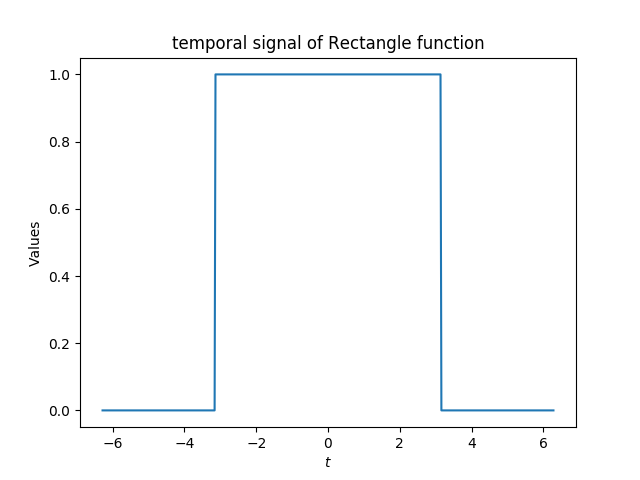
\includegraphics[width=0.45\textwidth]{python/Rectangular-Wave.png}
     \label{fig:SGD_1_single}}
     \quad 
     \subfigure[DFFT of $f(t)$]{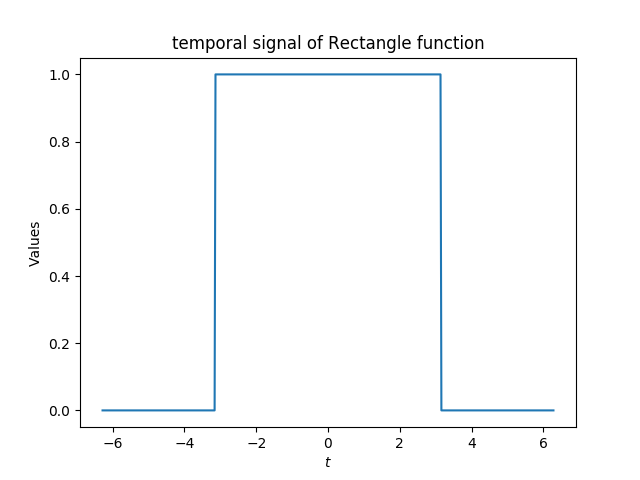
\includegraphics[width=0.45\textwidth]{python/Rectangular-Wave.png}
     \label{fig:SGD_1_single}} \\
     \subfigure[ $
     \widehat{f}(\lambda)$]{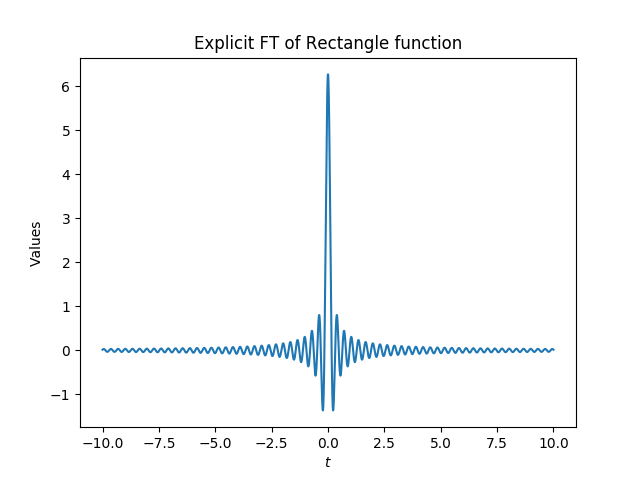
\includegraphics[width=0.45\textwidth]{python/ft-rectangle.png}
     \label{fig:SGD_1_single}}
 \end{figure*}


\end{exmp}


\begin{exmp}[$\cos(3t)$]
    
\begin{figure*}
     \centering 
    \subfigure[$\cos(3t)$]{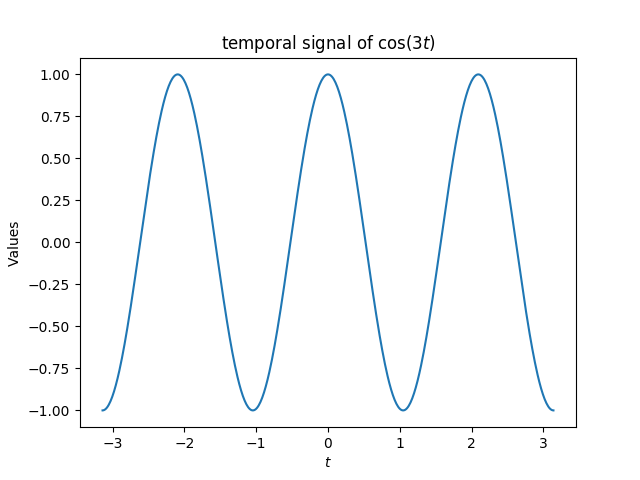
\includegraphics[width=0.45\textwidth]{python/cos3t.png}
     \label{fig:SGD_1_single}}
     \quad 
     \subfigure[DFFT of
     $f(t)$]{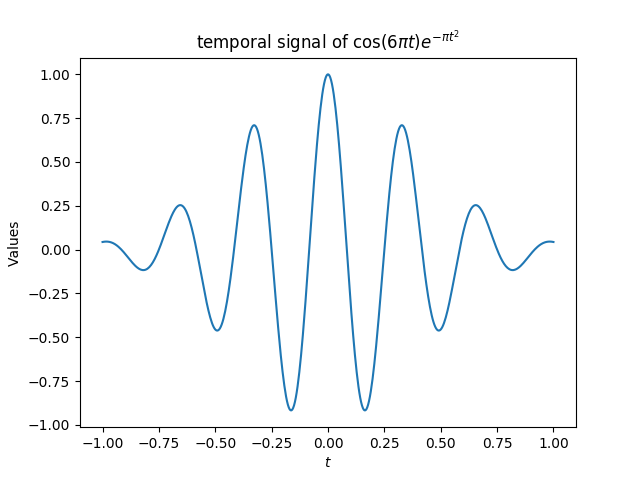
\includegraphics[width=0.45\textwidth]{python/cos-exp.png}
     \label{fig:SGD_1_single}} \\
     \subfigure[ $
     \widehat{f}(\lambda)$]{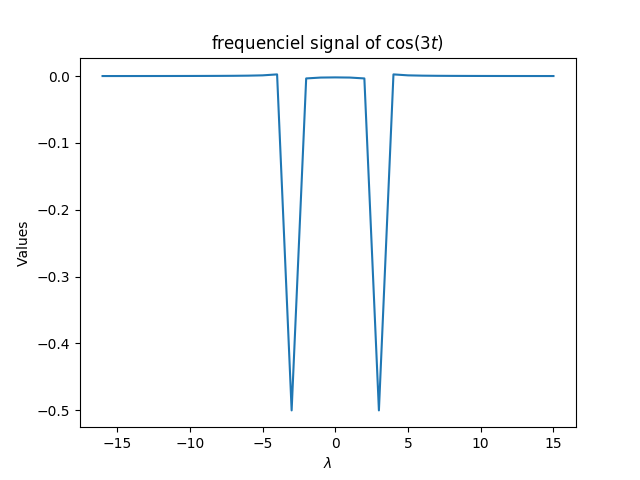
\includegraphics[width=0.45\textwidth]{python/fftcos3t.png}
     \label{fig:SGD_1_single}}
 \end{figure*}
\end{exmp}


\begin{exmp}[$\cos(6\pi t)e^{-\pi t^2}$]

\begin{figure*}
     \centering 
    \subfigure[Rectangle Function $f(t)$]{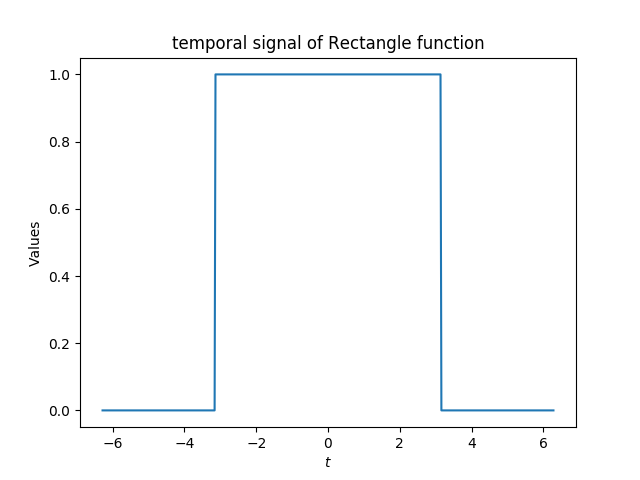
\includegraphics[width=0.45\textwidth]{python/Rectangular-Wave.png}
     \label{fig:SGD_1_single}}
     \quad 
     \subfigure[DFFT of $f(t)$]{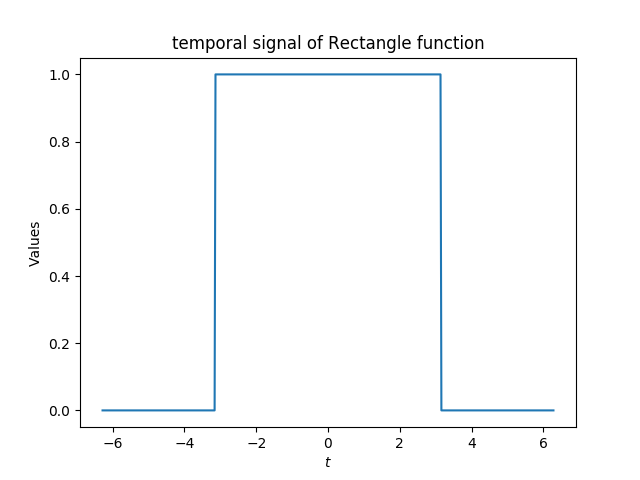
\includegraphics[width=0.45\textwidth]{python/Rectangular-Wave.png}
     \label{fig:SGD_1_single}} \\
     \subfigure[ $
     \widehat{f}(\lambda)$]{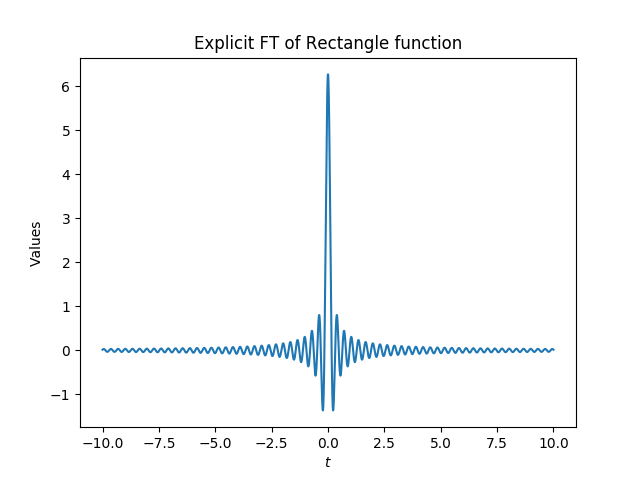
\includegraphics[width=0.45\textwidth]{python/ft-rectangle.png}
     \label{fig:SGD_1_single}}
 \end{figure*}
    
\end{exmp}

























\newpage

What is $ f_n  = f\left( \frac{ kT _{ \text{obs}  }^{  }  }{ N } \right)  $.  and what is
it to mean that the step is always 1/T for the DFT? 
